\documentclass{beamer}
\usepackage{multicol}

\definecolor{darkturquoise}{rgb}{0.0, 0.81, 0.82}
\usetheme[progressbar=frametitle]{metropolis} % https://hartwork.org/beamer-theme-matrix/
\setbeamertemplate{frame numbering}[fraction]
\useoutertheme{metropolis}
\useinnertheme{metropolis}
\usefonttheme{metropolis}
\usecolortheme{spruce}
\setbeamercolor{background canvas}{bg=white}

\title{\LaTeX\ Beamer Tutorial}
\subtitle{Functions, Limits and Derivatives}
\author{Joel Brigida}
\institute{Florida Atlantic University}
\date{}

\setbeamercovered{transparent=5} % Hidden text on slides is somewhat visible

\begin{document}
\metroset{block=fill} % display texts in colored blocks

\begin{frame}
    \titlepage
\end{frame}

\begin{frame}[t]{Functions} \vspace{1cm}
    \begin{block}{Definition Of A Function}
        \vspace{6pt}
        A \textbf{function} $f$ is a rule that assigns each element $x$ in a set $D$ exactly one element, called $f(x)$, in a set $E$.
        \vspace{6pt}
    \end{block}
    \vspace{6pt}
    Set $D$ is called the 
    \only<1>{\line(1,0){50}}
    \only<2>{\textcolor{magenta}{domain}}
    \, of the function.\\[10pt]

    Set $E$ is called the
    \only<1>{\line(1,0){50}}
    \only<2>{\textcolor{magenta}{range}}
    \, of the function.\\[10pt]

\end{frame}

\begin{frame}{Your Very First Flash Card} \vspace{10pt}
    \begin{columns}[onlytextwidth]
        \column{0.4 \textwidth}
        $\sqrt{x^2} =$
        \begin{enumerate}[a)]
            \item $x$
            \item $-x$
            \item $|x|$
            \item undefined
        \end{enumerate}
        \column{0.6 \textwidth}
        \only<3>{ % only displays on slide 3
        $\sqrt{x^2} = 
        \begin{cases}
            -x, & x < 0 \\
            x, & x \geq 0
        \end{cases}$} \\[10pt]
        \only<2->{ % displays on slide 2 and beyond
        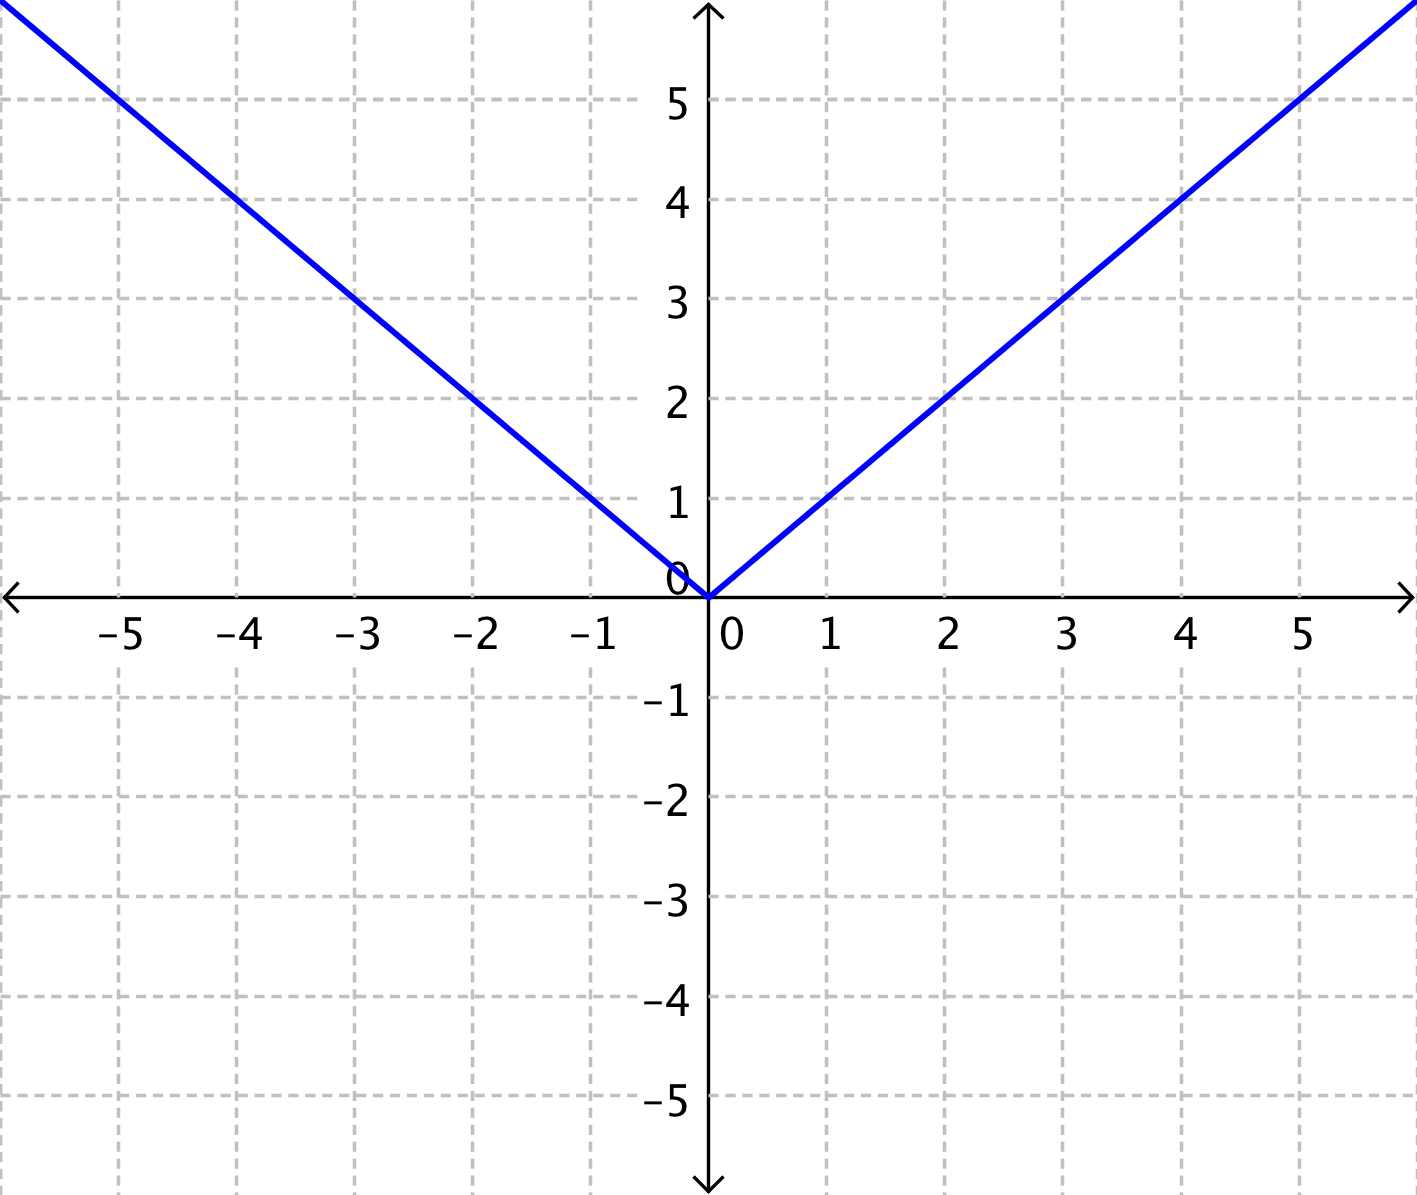
\includegraphics[scale=0.45]{xsquared}}
    \end{columns}
\end{frame}

\begin{frame}[t]{Parent Functions} \vspace{6pt} \large
    You should be able to identify by name and sketch a graph of each of the following parent functions:
    \begin{enumerate}
        \begin{multicols}{3} % Automatically Format to 3 columns
            \item $y = x$
            \item $y = |x|$
            \item $y = x^2$
            \item $y = x^3$
            \item $y = x^b$
            \onslide<2->{ % only displays on slide 2 and beyond
            \item $y = \sqrt{x}$
            \item $y = \sqrt[3]{x}$
            \item $y = \frac{1}{x}$
            \item $y = 2^x$
            \item $y = e^x$ }
            \onslide<3->{ % Only displays on slide 3 and beyond
            \item $y = \ln(x)$
            \item $y = \frac{1}{1 + e^{-x}}$
            \item $y = \sin(x)$
            \item $y = \cos(x)$
            \item $y = \tan(x)$ }
        \end{multicols}
    \end{enumerate}    
\end{frame}

\begin{frame}[standout]
    \begin{flushleft}
        Thank You For Attending.\\[6pt]
        \begin{small}
            Contact Info:\\
            Joel Brigida
        \end{small}
        
    \end{flushleft}
\end{frame}

\end{document}